\documentclass[final,12pt]{colt2018} % Anonymized submission
% \documentclass{colt2017} % Include author names

% The following packages will be automatically loaded:
% amsmath, amssymb, natbib, graphicx, url, algorithm2e

%\usepackage{graphpap,amscd,mathrsfs,graphicx,lscape,enumitem,dsfont,bm,url,subfigure}
%\usepackage{epsfig,amstext,xspace}
%\usepackage{algorithm,algorithmic,comment}
\usepackage{enumerate}
%\usepackage{thmtools,thm-restate}

%\documentclass[anon,12pt]{colt2017} 
 
\newcommand{\E}{\mathbf{E}}
\usepackage{enumerate}
%\usepackage{algorithm,algorithmic}
\usepackage{auxiliary}
%\usepackage[utf8]{inputenc} % allow utf-8 input
%\usepackage[T1]{fontenc}    % use 8-bit T1 fonts
%\usepackage{hyperref}       % hyperlinks
\usepackage{url}            % simple URL typesetting
\usepackage{booktabs}       % professional-quality tables
%\usepackage{amsfonts}       % blackboard math symbols
\usepackage{nicefrac}       % compact symbols for 1/2, etc.
\usepackage{microtype}      % microtypograpy
\usepackage{setspace}

\usepackage{color}              % Need the color package
%\usepackage{color-edits}
\usepackage[suppress]{color-edits}
\addauthor{tl}{cyan}
\addauthor{et}{blue}
\addauthor{ks}{brown}

% Short version on
%   \newcommand{\shortversion}[1]{#1}   \newcommand{\longversion}[1]{}
% 
% Long version on
\newcommand{\shortversion}[1]{} \newcommand{\longversion}[1]{#1}

\singlespacing
%\doublespacing

\newcommand{\F}{\mathcal{F}}

\title[Small-loss bounds for online learning with partial information]{Small-loss bounds for online learning with partial information\\(Extended abstract)}
\usepackage{times}
 % Use \Name{Author Name} to specify the name.
 % If the surname contains spaces, enclose the surname
 % in braces, e.g. \Name{John {Smith Jones}} similarly
 % if the name has a "von" part, e.g \Name{Jane {de Winter}}.
 % If the first letter in the forenames is a diacritic
 % enclose the diacritic in braces, e.g. \Name{{\'E}louise Smith}

 % Two authors with the same address
  % \coltauthor{\Name{Author Name1} \Email{abc@sample.com}\and
  %  \Name{Author Name2} \Email{xyz@sample.com}\\
  %  \addr Address}

 % Three or more authors with the same address:
 % \coltauthor{\Name{Author Name1} \Email{an1@sample.com}\\
 %  \Name{Author Name2} \Email{an2@sample.com}\\
 %  \Name{Author Name3} \Email{an3@sample.com}\\
 %  \addr Address}


 % Authors with different addresses:
 \coltauthor{\Name{Thodoris Lykouris} \Email{teddlyk@cs.cornell.edu}\\
 \addr 107 Hoy Rd, Ithaca, NY, 14850
 \AND
 \Name{Karthik Sridharan} \Email{sridharan@cs.cornell.edu}\\
 \addr 107 Hoy Rd, Ithaca, NY, 14850
 \AND
 \Name{\'Eva Tardos} \Email{eva.tardos@cornell.edu}\\
 \addr 107 Hoy Rd, Ithaca, NY, 14850
  }

\begin{document}

\maketitle

\begin{abstract}
We present preconditioned stochastic gradient descent (SGD) algorithms for the $\ell_1$ minimization problem $\min_{\xx}\|\AA \xx - \bb\|_1$ in the overdetermined case, where there are far more constraints than variables. Specifically, we have $\AA \in \R^{n \times d}$ for $n \gg d$. Commonly known as the Least Absolute Deviations problem, $\ell_1$ regression can be used to solve many important combinatorial problems, such as minimum cut and shortest path. SGD-based algorithms are appealing for their simplicity and practical efficiency.
% Our algorithms precondition the matrix $\AA$ and then solve the problem for the resulting matrix $\tilde{\AA}$ using gradient descent techniques.
Our primary insight is that careful preprocessing can yield preconditioned matrices $\tilde{\AA}$ with strong properties (besides good condition number and low-dimension) that allow for faster convergence of gradient descent. In particular, we precondition using Lewis weights to obtain an isotropic matrix with fewer rows and strong upper bounds on all row norms. We leverage these conditions to find a good initialization, which we use along with recent smoothing reductions and accelerated stochastic gradient descent algorithms to achieve $\epsilon$ relative error in $\Otil(nnz(\AA) + d^{2.5} \epsilon^{-2})$ time with high probability, where $nnz(\AA)$ is the number of non-zeros in $\AA$. This improves over the previous best result using gradient descent for $\ell_1$ regression. We also match the best known running times for interior point methods in several settings.

Finally, we also show that if our original matrix $\AA$ is approximately isotropic and the row norms are approximately equal, we can give an algorithm that avoids using fast matrix multiplication and obtains a running time of $\Otil(nnz(\AA) + s d^{1.5}\epsilon^{-2} + d^2\epsilon^{-2})$, where $s$ is the maximum number of non-zeros in a row of $\AA$. In this setting, we beat the best interior point methods for certain parameter regimes.


%We consider the $\ell_1$ minimization problem $\min_{\xx}||\AA \xx - \bb||_1$ in the overconstrained case, where there are far more constraints than variables. More specifically, we have $\AA \in \R^{n \times d}$ for $n \gg d$. By using Lewis Weights preconditioning on $\AA$ and a careful initialization, we show that a standard stochastic gradient descent algorithm achieves $\epsilon$ relative error in about $nnz(\AA) +  d^3\epsilon^{-2}$ time with high probability. If we leverage smoothing reductions in \cite{AllenZhuH16} and the accelerated stochastic gradient descent algorithms in \cite{AllenZhu17}, we can achieve a running time of about $nnz(\AA) + d^{2.5}\epsilon^{-2}$ with the same guarantees. Both of these running times improve over the previous results in \cite{YangCRM16} and the latter result is comparable to the best known running times for interior point methods \cite{LeeS15}.
%
%The key idea will be to use our preconditioning to restrict our consideration to matrices $\AA$ such that $\AA^T\AA = \II$ and every row norm of $\AA$ is upper bounded by $O(\sqrt{d/n})$. \cite{cohenpeng} show that sampling $\AA$ with Lewis weights takes about $nnz(\AA) +d^{\omega}$ time and approximately preserves the minimization problem. Moreover, we can assume $n\le O(d\epsilon^{-2}\log n)$ for the sampled matrix. We then prove that all leverage scores of the sampled matrix are approximately equal. Since rotations preserve leverage scores, we can then rotate our sampled matrix to ensure that our desired properties are met in about $d^{\omega}\epsilon^{-2}$ time.
%
%Finally, we also show that if our original matrix $\AA$ is such that $\AA^T\AA \approx \II$ and the row norms of $\AA$ are bounded, we can avoid using fast matrix multiplication and prove a running time of about $nnz(\AA) + s d^{1.5}\epsilon^{-2}$, where $s$ is the maximum number of non-zeros in a row of $\AA$.

%Consequently, we will be able to restrict our consideration to matrices $A$ such that $A^TA \approx I$, and all row norms are equal, which is to say $||A_{i,:}||_2 = \sqrt{\frac{d}{n}}$ for all $i$.
%
%With a careful choice of our initial $x$, we show that standard gradient descent and stochastic gradient descent algorithms under these further assumptions only require $O(\frac{d}{\epsilon^2})$ and $O(\frac{d^2}{\epsilon^2})$ iterations, respectively, to achieve $\epsilon$ relative error with respect to the minimum objective value. Accordingly, these methods each achieve respective total runtime of $O(\frac{md}{\epsilon^2})$ and $O(\frac{d^3}{\epsilon^2})$, along with an $O(m)$ preconditioning cost, improving over the previous results in \cite{MahoneySGD}.
%
%We further examine the consequences of our assumptions when combined with smoothing reductions in [cite] and accelerated gradient descent techniques in [cite,cite]. As a result we are able to further improve the running times to $O(\frac{md}{\epsilon})$ and $O(dn\log{1/\epsilon} + \frac{d^2\sqrt{n}}{\epsilon})$.
%
%Random sampling $d\epsilon^{-2}\log{d}$ rows of $A$ will only incur error $\epsilon$ and reduces the latter running time to $O(\frac{d^{2.5}\log{d}}{\epsilon^2})$, which is then comparable to interior point methods of [cite]

\end{abstract}

\begin{keywords}
Online Learning, Bandits, Feedback Graphs, Regret, High probability
\end{keywords}

\section{Introduction}

% !TeX root = main.tex
\section{Introduction}
\label{sec:intro}
Generative models are often trained in an unsupervised fashion, fitting a model $q$ to a set of observed data $x_P \subseteq X$ drawn iid from some true distribution $p$ on $x\in X$. Now, of course $p$ may not exactly belong to family $Q$ of probability distributions being fit, whether $Q$ consists of Gaussians mixture models, Markov models, or even neural networks of bounded size. We first discuss the limitations of generative modeling without feedback, and then discuss our model and results.

%\subsection{Limitations of Generative Modeling from Positive Examples Alone}
Consider fitting a generative model on a text corpus consisting partly of poetry written by four-year-olds and partly of mathematical publications from the {\em Annals of Mathematics}. Suppose that learning to generate a poem that looks like it was written by a child was easier than learning to generate a novel mathematical article with a correct, nontrivial statement. If the generative model pays a high price for generating unrealistic examples, then it may be better off learning to generate children's poetry than mathematical publications. However, without negative feedback, it may be difficult for a neural network or any other model to know that the mathematical articles it is generating are stylistically similar to the mathematical publications but do not contain valid proofs.\footnote{This is excluding clearly fake articles published without proper review in lower-tier venues \citep{LabbeL13}.} 

As a simpler example, the classic Markovian ``trigram model'' of natural language assigns each word a fixed probability conditioned only on the previous two words. Prior to recent advances in deep learning, for decades the trigram model and its variant were the workhorses of language modeling, assigning much greater likelihood to natural language corpora than numerous linguistically motivated grammars and other attempts \citep{Rosenfeld00}. However, text sampled from a trigram is typically nonsensical, e.g., the following text was randomly generated from a trigram model fit on a corpus of text from the Wall Street Journal \citep{JurafskyM09}:
\begin{quote}
They also point to ninety nine point six billion dollars from two hundred
four oh six three percent of the rates of interest stores as Mexico and
gram Brazil on market conditions. 
\end{quote}

In some applications, like text compression using a language model \citep{WittenNC87}, maximizing likelihood is equivalent to optimizing compression. However, in many  applications involving generation, such nonsense is costly and unacceptable. Now, of course it is possible to always generate valid data by returning random training examples, but this is simply overfitting and not learning. Alternatively, one could incorporate human-in-the-loop feedback such as through crowdsourcing, into the generative model to determine what is a valid, plausible sentence.

In some domains, validity could be determined automatically. Consider a Markovian model of a well-defined concept such as mathematical formulas that compile in \LaTeX{}. Now, consider a $n$-gram Markovian character model which the probability of each subsequent character is determined by the previous $n$ characters. For instance, the expression \$\{2+\{x-y\}\$ is invalid in \LaTeX{} due to mismatched braces. For this problem, a \LaTeX{} compiler may serve as a validity oracle. Various $n$-gram models can be fit which only generate valid formulas. To address mismatched braces, for example, one such model would ensure that it always closed braces within $n$ characters of opening, and had no nested braces. While an $n$-gram model will not perfectly model the true distribution over valid \LaTeX{} formulas, for certain generative purposes one may prefer an $n$-gram model that generates valid formulas over one that assigns greater likelihood to the training data but generates invalid formulas. 

Figure \ref{fig:rectangle} illustrates a simple case of learning a rectangle model for data which is not uniform over a rectangle. A maximum likelihood model would necessarily be the smallest rectangle containing all the data, but most examples generated from this distribution may be invalid. Instead a smaller rectangle, as illustrated in the figure, may be desired.

\begin{figure}[h]\label{fig:rectangle}
\centering
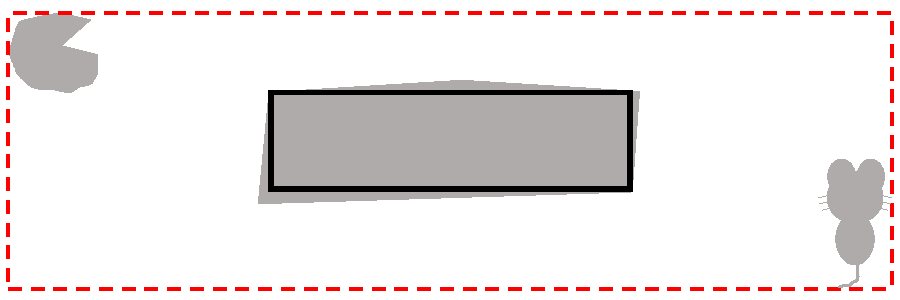
\includegraphics[width=3in]{fig.pdf}
\caption{Example where the underlying distribution $p$ is uniform over the (gray) valid regions. The solid rectangle maximizes our objective since it does not output nonsense (is supported only within the grey matter) and is closest to the $p$ (covers the maximum amount of grey matter). In contrast, the standard maximum likelihood (dashed red) rectangle must fully contain the observed samples, thus generating invalid points most of the time.  }
\end{figure}

Motivated by these observations, we evaluate a generative model $q$ on two axes. First is {\em coverage}, which is related to the probability assigned to future examples drawn from the true distribution $p$. Second is {\em validity}, defined as the probability that random examples generated from $q$ meet some validity requirement. Formally, we measure coverage in terms of a bounded {\em loss}:
$$\Loss(p,q)=\E_{x \sim p}[L(q_x)],$$
where $L:[0,1]\rightarrow [0,M]$ is a bounded decreasing function such as the capped log-loss $L(q_x)=\min(M, \log 1/q_x)$. % or $L(q_x)=\log 1/(q_x+\exp(-M))$. 
A bounded loss has the advantages of being efficiently estimable, and also it enables a model to assign 0 probability to one example (e.g., an outlier or error) if it greatly increases the likelihood of all other data. Validity is defined with respect to a set $V \subseteq X$, and $q(V)$ is the probability that a random example generated from $q$ lies within $V$. 

Clearly, there is a tradeoff between coverage and validity. We first focus on the case of (near) perfect validity. A Valid Generative Modeling (VGM) algorithm if it outputs, for a family of distributions $Q$ over $X$, if it outputs $\hat{q}$ with (nearly) perfect validity and whose loss is nearly as good as the loss of the best valid $q\in Q$. More precisely, $A$ is a VGM learner of $Q$ if for any nonempty valid subset $V \subseteq X$, any probability distribution $p$ over $V$, and any $\eps>0$, $A$ uses $n$ random samples from $p$ and makes $m$ membership oracle calls to $V$ and outputs a distribution $\hat{q}$ such that, $$\Loss(p, \hat{q}) \leq \min_{q \in Q: q(V)=1}\Loss(p,q) + \eps ~\text{ and }~\hat{q}(V)\geq 1-\eps.$$ 
We aim for our learner to be sample and query efficient, requiring that $n$ and $m$ are polynomial in $M, 1/\eps$ and a measure of complexity of our distribution class $Q$.
Furthermore, we would like our algorithms to be computationally efficient, with a runtime polynomial in the size of the data, namely the $n + m$ training examples. 
A more formal description of the problem is available in Section~\ref{sec:problem}.

$A$ is said to be {\em proper} if it always outputs $\hat{q}\in Q$ and {\em improper} otherwise.
In Section~\ref{sec:impossibility}, we first show that efficient proper learning for VGM is impossible. This is an information-theoretic result, meaning that even given infinite runtime and positive samples, one still cannot solve the VGM problem. Interestingly, this is different from binary classification, where it is possible to statistically learn from iid examples without a membership oracle.

Our first main positive result is an efficient (improper) learner for VGM. The algorithm relies on a subroutine that solves the following {\em Generative Modeling with Negatives} (GMN) problem: given sets $X_P, X_N \subset X$ of positive and negative examples, find the probability distribution $q \in Q$ which minimizes $\sum_{x \in X_P} L(q(x))$ subject to the constraint that $q(X_N)=0$. For simplicity, we present our algorithm for the case that the distribution family $Q$ is finite, giving sample and query complexity bounds that are logarithmic in terms of $|Q|$. However, as we show in Section~\ref{sec:infinite-families}, all of our results extend to infinite families $Q$. It follows that if one has a computationally efficient algorithm for the GMN problem for a distribution family $Q$, then our reduction gives a computationally efficient VGM learning algorithm for $Q$.

Our second positive result is an algorithm that minimizes $\Loss(p,q)$ subject to a relaxed validity constraint comparing against the optimal distribution that has validity $q(V)$ at least $1-\alpha$ for some $\alpha>0$. We show in Section~\ref{sec:partial-validity} that even in this more general setting, it is possible to obtain an algorithm that is statistically efficient but may not be computationally efficient. An important open question is whether there exists a computationally efficient algorithm for this problem when given access to an optimization oracle, as was the case for our algorithm for VGM.

\subsection{Related Work}
\cite{KearnsMRRSS94} showed how to learn distributions from positive examples in the realizable setting, i.e., where the true distribution is assumed to belong to the class being learned. In the same sense as their work is similar to PAC learning \citet{Valiant84} of distributions, our work is like agnostic learning \citet{KearnsSS94} in which no assumption on the true distribution is made. 

Generative Adversarial Networks (GANs)~\cite{GoodfellowPMXWOCB14} are an approach for generative modeling from positive examples alone, in which a generative model is trained against a discriminator that aims to distinguish real data from generated data. In some domains, GANs have been shown to outperform other methods at generating realistic-looking examples. Several shortcomings of GANs have been observed \citet{AroraRZ18}, and GANs are still subject to the theoretical limitations we argue are inherent to any model trained without a validity oracle. 

In supervised learning, there is a rich history of learning theory with various types of queries, including membership which are not unlike our (in)validity oracle. Under various assumptions, queries have been shown to facilitate the learning of complex classes such as finite automata \citet{Angluin88} and DNFs \citet{Jackson97}. See the survey of \cite{Angluin92} for further details.  Interestingly, \cite{Feldman09} has shown that for agnostic learning, i.e., without making assumptions on the generating distribution, the addition of membership queries does not enhance what is learnable beyond random examples alone. 
Supervised learning also has a large literature around active learning, showing how the ability to query examples reduces the sample complexity of many algorithms. See the survey of \cite{Hanneke14}. Note that the aim here is typically to save examples and not to expand what is learnable.
 
More sophisticated models, e.g., involving neural networks, can mitigate the invalidity problem as they often generate more realistic natural language and have even been demonstrated to generate \LaTeX{} that nearly compiles \citep{Karpathy15} or nearly valid Wikipedia markdown. However, longer strings generated are unlikely to be valid. For example, \cite{Karpathy15} shows generated markdown which includes:
\begin{quote}
==Access to ''rap===
The current history of the BGA has been [[Vatican Oriolean Diet]], British Armenian, published in 1893.  While actualistic such conditions such as the [[Style Mark Romanians]] are still nearly not the loss.
\end{quote}

Even ignoring the mismatched quotes and equal signs, note that this example has two so-called ``red links'' to two pages that do not exist. Without checking, it was not obvious to us whether or not Wikipedia had pages titled {\em Vatican Oriolean Diet} or {\em Style Mark Romanians}. In some applications, one may or may not want to disallow red links. In the case that they are considered valid, one may seek a full generative model of what might plausibly occur inside of brackets, as the neural network has learned in this case. If they are disallowed, a model might memorize links it has seen but not generate new ones. A validity oracle can help the learner identify what it should avoid generating.

 In practice, \cite{KusnerPH17} discuss how generative models from neural networks (in particular autoencoders) often generate invalid sequences. 
\cite{JanzWPKH18} learn the validity of examples output by a generative model using oracle feedback. 


\subsection{Related work}
% !TEX root = main.tex
Online learning with partial information dates back to the seminal work of \cite{Lai1985}. They consider a stochastic version, where losses come from fixed distributions. We focus on the case where the losses are selected adversarially, i.e. they do not come from a distribution and may be adaptive to the algorithm's choices. This was first studied by \cite{Auer2003} who provided the EXP3 algorithm for pure bandits and the EXP4 algorithm for learning with expert advice (a generalization of the contextual bandits of \cite{Langford2007}). They focus on uniform regret bounds, i.e. that grow as a function of time $o(T)$, and bound mostly the expected performance, but such guarantees can also be derived with high probability \citep{Auer2003,AudibertB10,pmlr-v15-beygelzimer11a}. Data-dependent guarantees are easily derived from the above algorithms for the case of maximizing some reward  as even getting reward $0$ with probability of $\epsilon$ only causes an $\eps$ fraction of loss in utility. In contrast, incurring high cost with a small probability $\epsilon$ can dominate the loss of the algorithm, if the best arm has small loss. In this paper we develop 
data-dependent guarantees for partial information algorithm for the cases of losses. There are a few specialized algorithms that achieve such small-loss guarantees for the case of bandits for pseudo-regret, e.g. by ensuring that the estimated losses of all arms remain close \citep{Allenberg2006,Neu15_semibandits} or using a stronger regularizer \citep{RakhlinS13predictablesequences,FosterLLST16}, but all of these methods neither offer high probability small-loss guarantees even for the bandit setting, nor extend to graph-based feedback. Our technique allows us to develop small-loss bounds on actual regret with high probability. 

The graph-based
partial information that we examine in this paper 
was introduced by \cite{MannorS11} who provided ELP, a linear programming based algorithm achieving
$\widetilde{\bigO}{(\sqrt{\alpha T})}$ regret for undirected graphs. \cite{AlonCGM13,AlonCGMMS} provided variants of Exp3  (Exp3-SET) that recovered the previous bound via what they call \emph{explicit exploration}. Following this work, there have been multiple results on this setting, e.g.\citep{AlonCBDK15,Cohen2016, KocakNV16, tossou:aaai2017b}, but prior to our work, there was no small-loss guarantee for the feedback graph setting that could exploit the graph structure. To obtain a regret bound depending on the graph structure, the above techniques upper bound the losses of the arms by the maximum loss which results in a dependence on the time horizon $T$ instead of $L^{\star}$. Addressing this, we achieve regret that scales with an appropriate problem dimension, the size of the maximum independent set $\alpha$, instead of ignoring the extra information and only depending on the number of arms as all small-loss results of prior work.

Biased estimators have been used prior to our work for achieving better regret guarantees. The freezing technique of \cite{Allenberg2006} can be thought of as the first use of biased estimators.  Their \emph{GREEN} algorithm uses freezing in the context of the multiplicative weights algorithm for the case of pure bandits. Freezing keeps the range of estimated losses bounded and when used with the multiplicative weights algorithm, also keeps the cumulative estimated losses very close, which ensures that one does not lose much in the application of the full information algorithm. Using these facts, \cite{Allenberg2006} achieved small-loss guarantees for  pseudo-regret in the classical multi-armed bandit setting. 
An approach very close to freezing is the \emph{implicit exploration} of \cite{Kock2014EfficientLB} that adds a term in the denominator of the estimator making the estimator biased, even for the selected arms. 
The \emph{FPL-TrIX} algorithm of \cite{Neu15_semibandits} 
is based on the Follow the Perturbed Leader algorithm using implicit exploration together with truncating the perturbations to  guarantee that the estimated losses of all actions are close to each other and the \emph{geometric resampling} technique of \cite{NeuB13} to obtain these estimated losses. His analysis provides small-loss regret bounds for pseudo-regret, but does not extend to high-probability guarantees. The \emph{EXP3-IX} algorithm of  \cite{Kock2014EfficientLB}combines implicit exploration with multiplicative weights to obtain, via the analysis of \cite{Neu2015_implicit}, high-probability uniform bounds. Focusing on uniform regret bounds, exploration and truncation were presented as strictly superior to freezing. In this paper, we show an important benefit of the freezing technique: it can be extended to handle feedback graphs (via our dual-thresholding).
We also combine freezing with multiplicative weights to develop an algorithm we term \emph{GREEN-IX} which achieves optimal high-probability small-loss
$\widetilde{\bigO}(\sqrt{d L^{\star}})$ for the pure bandit setting. Finally, combining freezing with the truncation idea, we obtain the corresponding result for semi-bandits; in contrast, the geometric resampling analysis does not seem to extend to high probability since it does not provide a handle on the variance of the estimated loss. 

% This is where the content of your camera-copy paper goes.  Remember to:
% \begin{itemize}
% \item Limit the main text (without references and appendices) to 12 PMLR-formatted pages (i.e., using this template).
% \item Include, either in the main text or the appendices, all details, proofs
%   and derivations required to substantiate the results.
% \item Include {\em in the main text} enough details, including proof
%   details, to convince the reviewers of the contribution, novelty and significance of the submissions.
%   \end{itemize}



\subsection*{Full version}
We refer the reader to the full version of the paper that can be found here \url{https://arxiv.org/abs/1711.03639}.

% Acknowledgments---Will not appear in anonymized version
\acks{We thank Haipeng Luo for pointing out the connection 
to the contextual bandit setting, Jake Abernethy, Adam Kalai, and Santosh Vempala for a useful discussion about Follow the Perturbed Leader, and anonymous reviewers for their useful feedback. This work was supported by NSF grants CCF-1563714 and CDS\&E-MSS 1521544, and an NSF-CAREER Award 1750575 }

\bibliography{bib1}

\end{document}
